\documentclass{HGBAbgabe}
\usepackage[colorlinks]{hyperref}
\usepackage{tikz}

\begin{document}
	
	\HGBPdf{Angabe.pdf}{
		\begin{tikzpicture}[remember picture, overlay,x=1cm,y=-1cm]
			\node[draw=none,text width=6. cm,align=left] at (6.2,3.05) {Max Mustermann};
			\node[draw=none,text width=6. cm,align=left] at (6.2,3.65) {123456789};
			\node[draw=none,text width=1.8 cm,align=center] at (4.2,4.25) {2};
			\node[draw=none,text width=1.8 cm,align=center] at (4.2,4.85) {6h};
		\end{tikzpicture}
    }
    
	\tableofcontents

	\HGBSourceToc{}
	\pagebreak
	
\section{Verbatim}

\HGBVerbatim{example.h} 

\section{Module}

\HGBCppModule{example}

\section{Source}

\HGBCppSource{example.cpp}

\section{Image}

\begin{figure}
	\centering
	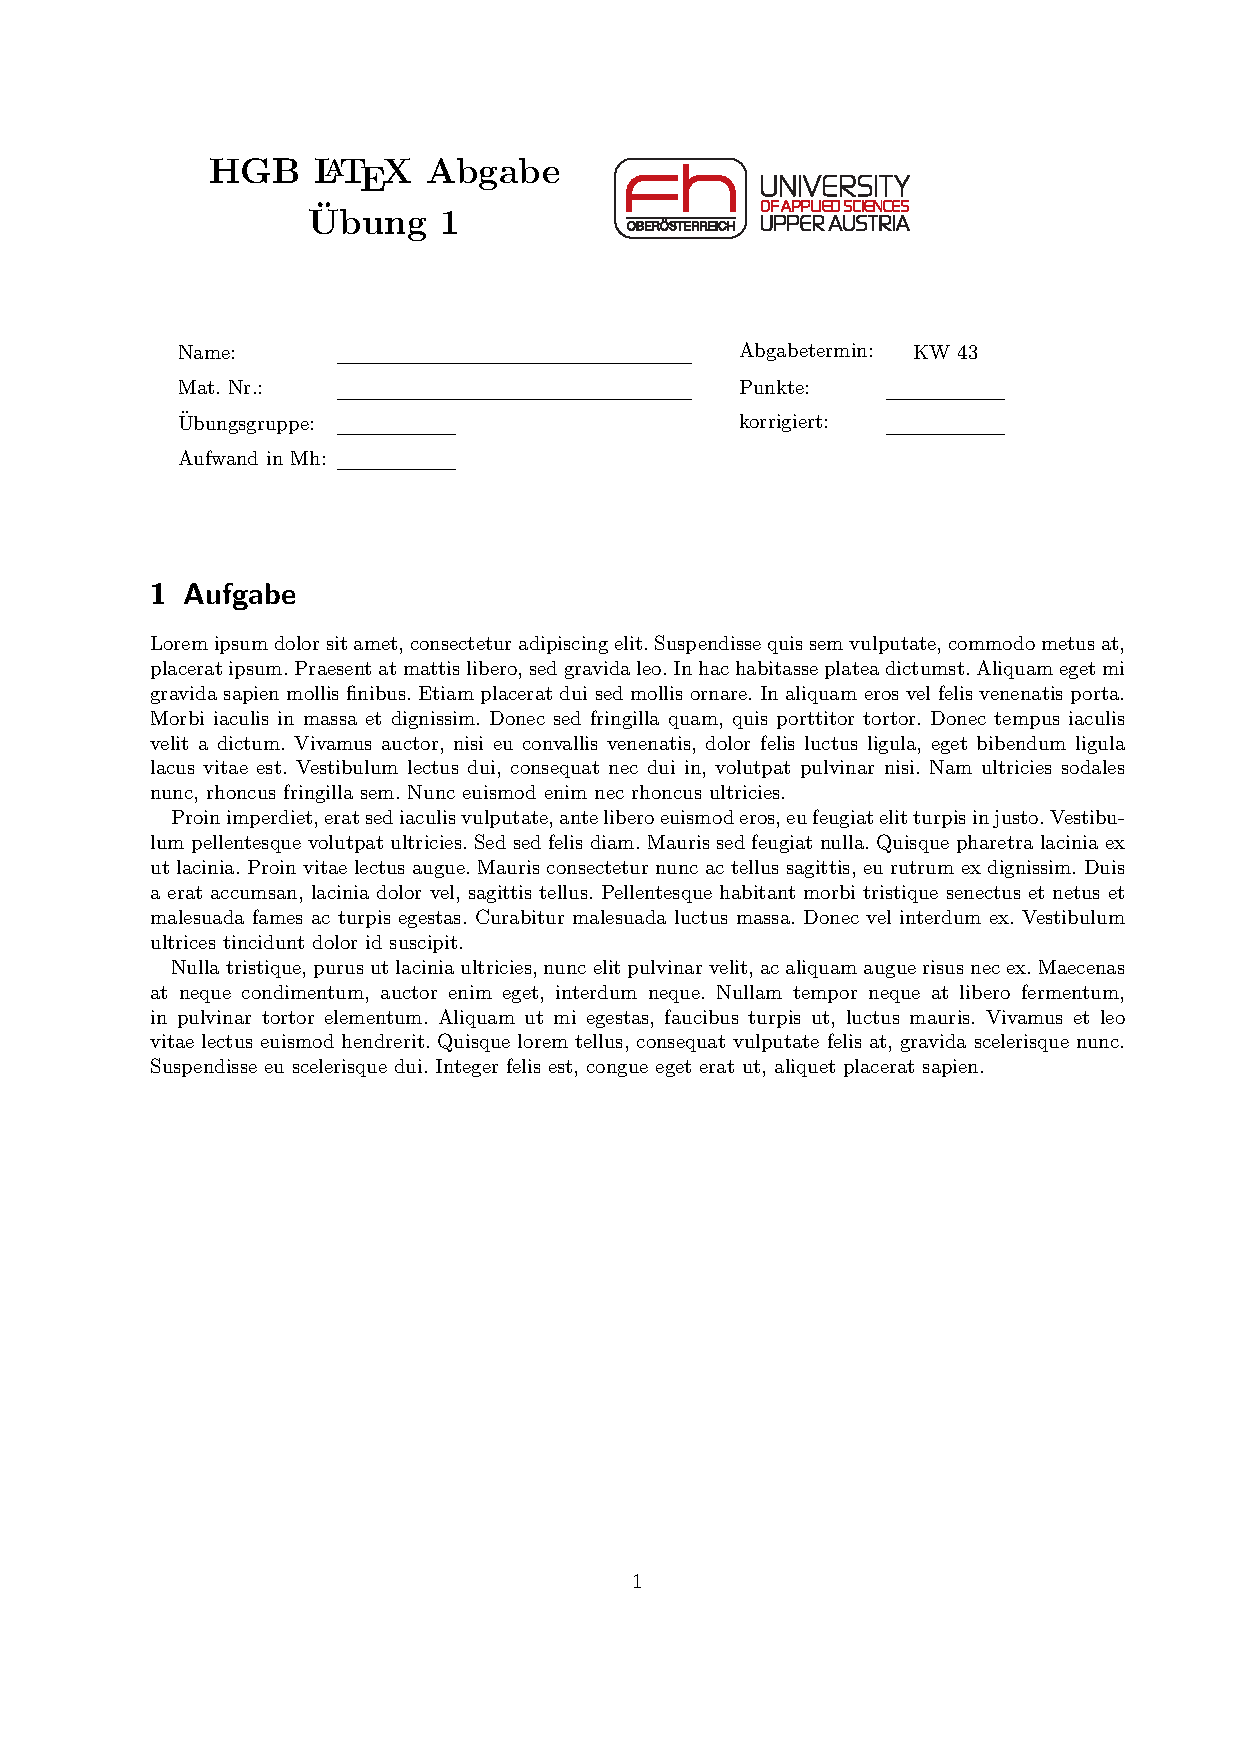
\includegraphics[width=0.4\linewidth]{Angabe.pdf}
	\caption{The logo in use}
	\label{fig:logo}
\end{figure}

Take a look at the nice exercise in \autoref{fig:logo}!

\end{document}
